%-------------------------------------------------------------------------------
%                            BAB II
%               TINJAUAN PUSTAKA DAN DASAR TEORI
%-------------------------------------------------------------------------------
%\fancyhf{}
% \fancyfoot[C]{\thepage}
\chapter{TINJAUAN KEPUSTAKAAN}
% \thispagestyle{plain} % Halaman pertama bab menggunakan gaya plain



% \par Untuk mendukung penelitian ini, maka dalam bab ini akan dikemukakan beberapa rumusan teori pendukung yang dikutip dari berbagai referensi baik dalam bentuk buku, artikel, maupun tulisan karya ilmiah lainnya termasuk hasil penelitian sebelumnya yang ada kaitannya dengan penelitian yang dilakukan.

% Mengatur format untuk bagian (section)


\section{Citra Medis}


\par Citra adalah gambaran dari suatu objek yang bisa kita lihat. Citra analog tidak bisa disimpan secara langsung dalam komputer. Oleh karena itu, kita perlu mengubah citra analog menjadi citra digital agar bisa diolah oleh komputer. Citra digital adalah citra yang bisa diolah menggunakan perangkat komputer. Alasan utama citra analog tidak bisa diolah oleh komputer adalah karena citra analog tidak memiliki konsep sampling dan kuantisasi. Konsep sampling adalah suatu metode yang mengubah citra analog menjadi \textit{grid} berbentuk M baris dan N kolom, sehingga citra menjadi lebih tersegmentasi. Semakin besar nilai M dan N, semakin halus citra digital yang dihasilkan. Sedangkan konsep kuantisasi adalah suatu metode yang mengubah intensitas dari citra analog menjadi intensitas diskrit. Baik sampling maupun kuantisasi memegang peranan penting dalam mengambil potongan citra menjadi bentuk M baris dan N kolom (proses sampling) serta menentukan nilai intensitas yang terdapat pada setiap titik tersebut (proses kuantisasi). Hasil akhir dari kedua konsep ini adalah citra yang memiliki resolusi sesuai dengan yang kita inginkan \citep{andono2018pengolahan}.

\par Dalam ilmu pengolahan citra, beragam jenis citra ada, dan salah satunya adalah citra \textit{Red Green Blue} (RGB), juga disebut sebagai citra \textit{true color}. Citra ini memiliki matriks data berukuran $m \times n \times 3$, yang menggambarkan warna merah, hijau, dan biru pada setiap piksel. Rentang nilai untuk setiap warna adalah antara 0 (nilai minimum) hingga 255 (nilai maksimum) dalam monitor komputer. Pada bagian ini, skala 0 hingga 255 dipilih berdasarkan representasi delapan digit dalam bilangan biner yang digunakan oleh komputer. Dengan demikian, lebih dari 16 juta warna dapat dihasilkan secara total. Penentuan warna pada setiap piksel didasarkan pada tingkat kecerahan merah, hijau, dan biru \citep{ardiansyah2013pengenalan}.

\par Di bidang kesehatan, pencitraan medis memegang peranan penting dalam berbagai bidang klinis seperti prosedur medis yang digunakan untuk deteksi dini, pemantauan, diagnosis, dan evaluasi pengobatan berbagai kondisi medis \citep{puttagunta2021medical}. Citra medis merujuk pada gambar dua dimensi yang menggambarkan struktur internal tubuh manusia, dimanfaatkan oleh profesional kesehatan untuk diagnosis penyakit. Pengolahan citra medis memiliki aplikasi luas, termasuk deteksi tumor atau kanker pada organ reproduksi wanita, identifikasi patologi pada organ-organ seperti paru-paru, hati, dan tulang, segmentasi struktur tulang dari jaringan otot, klasifikasi gigi, serta analisis gambar dari mikroskop. Berbagai teknologi digunakan dalam pencitraan medis ini, antara lain \textit{Magnetic Resonance Imaging} (MRI), \textit{X-Ray}, \textit{Ultrasonography} (USG), endoskopi, \textit{Computed Tomography} (CT-Scan), dan \textit{Nuclear Medicine} \citep{kusuma2018penerapan}. 

% Untuk memahami citra medis diperlukan bidang keilmuan yang mempelajari suatu asal usul penyakit yang disebut patologi \citep{cohnheim1889lectures}, dan bidang keilmuan yang mempelajari yang mempelajari cara mendiagnosa penyakit dengan menggunakan citra medis yang disebut radiologi \citep{wang2012machine}.

\section{\textit{Deep Learning}} 

\par \textit{Deep learning} adalah cabang ilmu \textit{machine learning} yang berbasis pada \textit{Artificial Neural Network} (ANN) sebagai pengembanganya. Metode dalam \textit{machine learning} biasanya hanya mengandalkan alat seperti \textit{Central Processing Unit} (CPU) dan \textit{Random Access Memory} (RAM) dalam menentukan kecepatan komputasi. Sedangkan metode \textit{deep learning} selain menggunakan CPU dan RAM, metode ini juga menggunakan \textit{Graphics Processing Unit} (GPU) sehingga proses komputasi data yang besar dapat dilakukan dengan cepat \citep{ilahiyah2018implementasi}.

\par \textit{Deep learning} memiliki pendekatan yang dapat dikategorikan seperti \textit{supervised learning}, \textit{unsupervised learning}, \textit{semi-supervised learning}, dan \textit{reinforcement learning} \citep{alom2019state}. Kategori pendekatan \textit{deep learning} dapat dilihat pada Gambar \ref{pendekatan-deeplearning}.

\begin{figure}[H]
    \centering
    {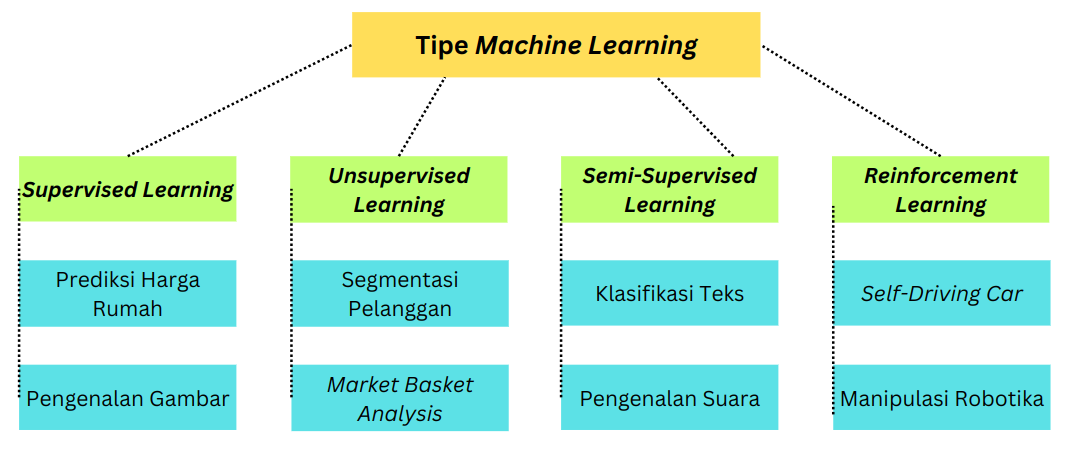
\includegraphics [width=\textwidth]{image/bab2/pendekatan-deep-learning.png}}
    \caption{Kategori pendekatan \textit{deep learning}}
    \label{pendekatan-deeplearning}
\end{figure}


\par Pendekatan ini melibatkan berbagai teknik dan algoritma untuk menyelesaikan berbagai jenis masalah. Dalam mengimplementasikan model \textit{deep learning}, beberapa \textit{hyperparameter} yang sangat penting untuk diperhatikan adalah \textit{learning rate}, \textit{batch size}, jumlah \textit{epochs}, dan arsitektur jaringan itu sendiri. \textit{Learning rate} adalah ukuran yang menentukan seberapa besar langkah yang diambil model saat memperbarui bobot selama pelatihan. \textit{Batch size} mengacu pada jumlah sampel data yang diproses sebelum memperbarui parameter model, sementara jumlah \textit{epochs} menunjukkan berapa kali seluruh \textit{dataset} akan dilalui selama pelatihan. Pemilihan \textit{hyperparameter} sering kali dilakukan dengan fleksibilitas berdasarkan eksperimen dan kebutuhan spesifik dari proyek yang sedang dikerjakan. Tidak ada aturan tetap mengenai nilai-nilai spesifik yang harus dipilih untuk \textit{hyperparameter}. Seorang peneliti dapat mencoba berbagai nilai untuk menemukan kombinasi yang optimal. Metode seperti \textit{grid search} menunjukkan bahwa nilai-nilai \textit{hyperparameter} dapat dipilih secara bebas dalam rentang yang telah ditentukan \citep{bergstra2012random}.


\par \textit{Grid search} adalah metode pencarian \textit{hyperparameter} yang melibatkan pencarian melalui ruang \textit{hyperparameter} dengan mencoba setiap kombinasi yang mungkin dari nilai \textit{hyperparameter} yang telah ditentukan sebelumnya. Dengan \textit{grid search}, seorang peneliti membuat sebuah \textit{grid} dari \textit{hyperparameter} yang berbeda dan mengevaluasi model dengan setiap kombinasi yang ada di \textit{grid} tersebut \citep{bergstra2012random}. Pendekatan ini memastikan bahwa semua kombinasi yang mungkin diuji, meskipun bisa sangat memakan waktu dan sumber daya.



\par Pada bidang medis \textit{deep learning} digunakan untuk memproses citra medis seperti X-rays, CT, scan MRI (\textit{Magnetic Resonance Imaging}) dan lain-lain untuk mendiagnosa kondisi kesehatan \citep{kelleher2019deep}.

\subsection{\textit{Artificial Neural Network}}

\par \textit{Artificial Neural Network} (ANN) atau jaringan saraf tiruan adalah jaringan saraf yang memproses informasi dengan cara yang mirip dengan otak manusia \citep{kristiyanti2023machine}. \textit{Neural network} terdiri dari elemen pemrosesan sederhana yang disebut \textit{node} yang saling terhubung, mirip dengan cara kerja neuron dalam otak manusia. Kemampuan untuk melakukan pemrosesan dalam jaringan ini disimpan dalam koneksi antara \textit{node}, yang biasanya disebut sebagai \textit{weight}. Nilai-nilai \textit{weight} ini diperoloeh melalui proses pembelajaran atau adaptasi yang berdasarkan pada pola data yang dipelajari oleh ANN \citep{gurney1997introduction}.

\subsection{Fungsi Aktivasi}


\par Fungsi aktivasi dalam konteks jaringan saraf dapat diibaratkan dengan cara tubuh manusia merespon rangsangan dari lingkungan. Ketika seseorang menerima rangsangan eksternal, tubuhnya secara otomatis meresponsnya. Sebagai contoh, ketika tangan kita digigit, tubuh kita akan merespons dengan menolak atau melepaskan gigitan tersebut. Respons tubuh ini akan semakin intens jika rangsangan yang diterima semakin kuat. Dalam konteks algoritma jaringan saraf, respons tubuh ini analoginya digantikan oleh nilai bobot dan tingkat aktivasi yang tinggi. Pada persamaan \ref{eq: neural network sebelum fungsi aktivasi} menunjukkan persamaan dari jaringan saraf sebelum menggunakan fungsi aktivasi.

% rumus neural network sebelum fungsi aktivasi

\begin{equation}
    % Rumus neural network sebelum fungsi aktivasi
    y = \sum_{i=1}^n x_i w_i + b
    \label{eq: neural network sebelum fungsi aktivasi}
\end{equation}

\begin{itemize}

    \item $y$ adalah nilai keluaran dari jaringan saraf.
    \item $x_i$ adalah nilai \textit{input} dari jaringan saraf.
    \item $w_i$ adalah bobot dari setiap nilai \textit{input}.
    \item $b$ adalah bias dari jaringan saraf.

\end{itemize}

\par Ketika menerapkan fungsi aktivasi pada persamaan \ref{eq: neural network sebelum fungsi aktivasi}, maka persamaan akan berubah menjadi seperti yang ditunjukkan pada persamaan \ref{rumus-fungsi-aktivasi}.

% rumus fungsi aktivasi

\begin{equation}
    % Rumus fungsi aktivasi
    z = \textit{Act}(\sum_{i=1}^n x_i w_i + b)
    \label{rumus-fungsi-aktivasi}
\end{equation}

\begin{itemize}
    \item $z$ adalah nilai keluaran dari jaringan saraf setelah menggunakan fungsi aktivasi.
    \item $Act$ adalah fungsi aktivasi.
    \item $x_i$ adalah nilai \textit{input} dari jaringan saraf.
    \item $w_i$ adalah bobot dari setiap nilai \textit{input}.
    \item $b$ adalah bias dari jaringan saraf.
\end{itemize}

\par Persamaan \ref{rumus-fungsi-aktivasi} ini menunjukkan bahwa nilai keluaran $z$ akan bergantung pada fungsi aktivasi terhadap nilai prediksi yang dihasilkan dari perkalian nilai \textit{input} dan bobot \citep{kristiyanti2023machine}. 

\par Fungsi aktivasi adalah komponen penting dalam jaringan saraf tiruan yang mengatur bagaimana nilai hasil penjumlahan terbobot dari \textit{input} data diubah menjadi \textit{output} yang dikeluarkan oleh neuron dalam jaringan saraf. Fungsi aktivasi ini digunakan untuk menentukan apakah suatu neuron akan meneruskan nilai kalkulasinya ke neuron berikutnya, berdasarkan suatu nilai ambang tertentu. Fungsi ini juga sering disebut sebagai fungsi transfer karena memiliki kemampuan untuk mengubah data yang dihasilkan dari hasil penjumlahan terbobot pada suatu lapisan, yang kemudian akan diteruskan ke lapisan selanjutnya. Fungsi aktivasi bisa berupa fungsi linear atau fungsi non-linear tergantung pada tugas yang ingin diselesaikan, dan fungsi aktivasi ini dapat digunakan dalam berbagai hal seperti pengenalan objek dan klasifikasi \citep{nwankpa2018activation}.

\par Fungsi aktivasi perlu memiliki sifat diskriminatif, yang merupakan aspek yang penting karena memungkinkan penggunaan proses propagasi balik kesalahan dalam pelatihan jaringan. Salah satu fungsi aktivasi yang umum digunakan dalam konteks CNN adalah fungsi ReLU (\textit{Rectified Linear Unit}). Fungsi ini merupakan fungsi aktivasi yang mengubah seluruh isi nilai \textit{input} menjadi angka positif \citep{alzubaidi2021review}. Persamaan fungsi aktivasi ini dapat dilihat pada persamaan \ref{eq:relu}.

\begin{equation}
    % Rumus fungsi aktivasi ReLU
    f(x)_\text{ReLU} = \max(0, x)
    \label{eq:relu}
\end{equation}

\par Salah satu fungsi aktivasi yang digunakan dalam berbagai model mutakhir seperti GPT-3, BERT, dan sebagian besar model Transformer lainya adalah \textit{Gaussian Error Linear Unit} (GELU). Fungsi ini merupakan fungsi aktivasi yang menimbang \textit{input} berdasarkan persentilnya, daripada mengelompokkan \textit{input} berdasarkan tandanya seperti ReLU. Oleh karena itu, GELU dapat dikatakan lebih mulus dibandingkan ReLU. Hal ini memungkinkan GELU untuk lebih mudah memperkirakan fungsi yang rumit daripada ReLU atau ELU \citep{hendrycks2016gaussian}. Persamaan fungsi aktivasi ini dapat dilihat pada persamaan \ref{eq:gelu}.

\begin{equation}
    % Rumus fungsi aktivasi GELU
    \operatorname{GELU}(x)=x P(X \leq x)=x \Phi(x)=x \cdot \frac{1}{2}[1+\operatorname{erf}(x / \sqrt{2})]
    \label{eq:gelu}
\end{equation}

\begin{itemize}

    \item{$x$ adalah nilai \textit{input} dari fungsi aktivasi.}

    \item{$\Phi$ adalah \textit{Cumulative Distribution Function} (CDF) dari $x$.}

    \item{$\operatorname{erf}$ adalah fungsi kesalahan dari $x$.}


\end{itemize}


\par Salah satu fungsi aktivasi yang dapat digunakan untuk mengklasifikasi lebih dari dua kelas adalah fungsi aktivasi \textit{softmax}. Persamaan \ref{eq:softmax} menunjukkan persamaan dari fungsi aktivasi \textit{softmax}.

\begin{equation}
    f_j(Z) = \frac{e^{z_j}}{\sum_k e^{z_k}}
    \label{eq:softmax}
\end{equation}

\par Pada persamaan \ref{eq:softmax}, Notasi $f_j$ menunjukkan hasil fungsi pada setiap elemen ke-j pada vektor keluaran kelas. Argumen $z$ merupakan hipotesis yang diberikan oleh model pelatihan agar dapat diklasifikasi oleh fungsi \textit{softmax} \citep{ilahiyah2018implementasi}. 



\subsection{Fungsi \textit{loss}}

\par Fungsi \textit{loss} adalah salah satu fungsi pada \textit{Artificial Neural Network} (ANN) untuk melakukan perhitungan nilai \textit{error} atau kesalahan dari hasil prediksi dari suatu \textit{output} ANN \citep{zhang2016neural}. 

\par Fungsi \textit{loss} yang menghukum kesalahan probabilitas \textit{false negative} daripada \textit{false positive} adalah \textit{categorical cross entropy} \citep{ho2019real}. Persamaan \ref{eq:categorical_cross_entropy} menunjukkan persamaan dari \textit{categorical cross-entropy}. 

\begin{equation}
    J_{cce} = -\frac{1}{M} \sum_{k=1}^{K} \sum_{m=1}^{M} y_{m}^{k} \log_{(\theta} (x_{m}, k)
    \label{eq:categorical_cross_entropy}
\end{equation}

% keterangan rumus categorical cross entropy

\begin{itemize}

    \item $M$ adalah jumlah sampel data yang digunakan untuk pelatihan.
    \item $K$ adalah jumlah kelas yang ada pada data.
    \item $y_{m}^{k}$ adalah nilai target dari sampel data ke-$m$ pada kelas ke-$k$.
    \item $x$ adalah \textit{input} untuk contoh pelatihan ke-$m$.
    \item $H_\theta$ adalah bobot model \textit{neural network} $\theta$.
\end{itemize}



    

\subsection{Fungsi Optimasi}

\par Fungsi optimasi atau \textit{optimization function} dapat diartikan sebagai suatu fungsi yang berperan sebagai \textit{black box}, dimana fungsi ini menerima kesalahan sebagai input dan menghasilkan nilai bobot yang optimal untuk suatu model ANN \citep{li2017learning}.

\par Salah satu dari fungsi optimasi yang dapat digunakan dalam pengembangan model \textit{deep learning} adalah Adam (\textit{Adaptive Moment Estimation}). Adam adalah teknik optimasi untuk \textit{gradient descent}. Metode ini sangat efisien saat bekerja dengan masalah yang melibatkan banyak data atau parameter. Algoritma ini membutuhkan memori yang lebih sedikit dan efisien. Secara intuitif, Adam merupakan gabungan antara algoritma \textit{stochastic gradient descent momentum} dan \textit{RMSProp}. Secara eksperimen Adam adalah teknik optimasi terbaik dengan \textit{training cost} yang rendah menurut \citep{kingma2014adam}. Gambar \ref{fig:adam} menunjukkan perbandingan teknik optimasi Adam dengan teknik optimasi lainnya.

\begin{figure}[H]
    \centering
    {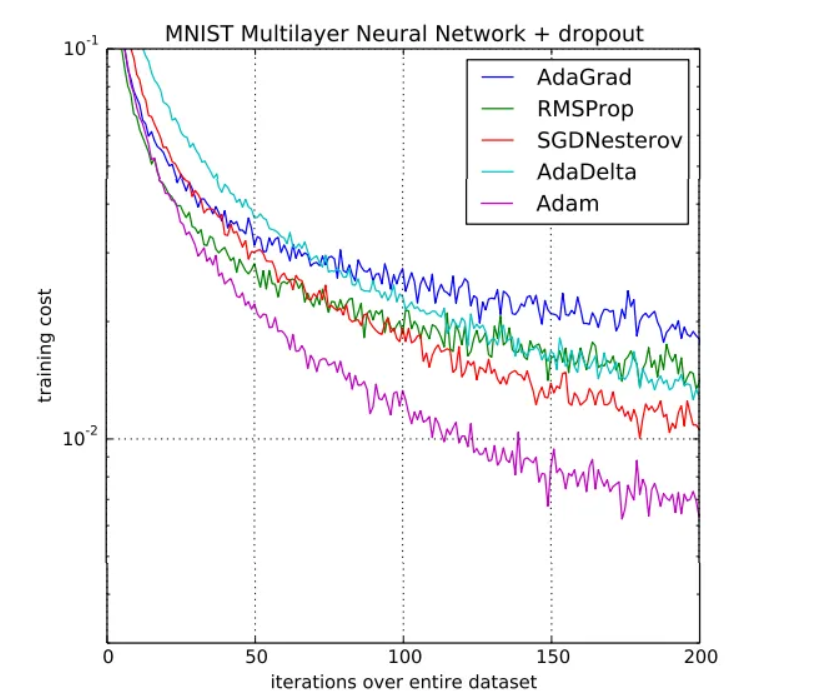
\includegraphics [width=\textwidth,height=8cm]{image/bab2/graf-optimisasi}}
    \caption{Perbandingan teknik optimasi Adam dengan teknik optimasi lainnya \citep{kingma2014adam}}
    \label{fig:adam}
\end{figure}


\section{\textit{Convolutional Neural Network}}

\par \textit{Convolutional Neural Network} (CNN) adalah turunan dari algoritma \textit{neural network} yang dikhususkan untuk memproses data yang berupa gambar. CNN adalah algoritma yang meniru proses pengolahan visual yang terjadi pada manusia. Seperti mata manusia yang berfungsi sebagai alat \textit{input}, CNN menggunakan lapisan konvolusi yang terdiri dari miliaran neuron untuk memproses informasi visual dan menghasilkan prediksi terhadap objek yang diamati \citep{kristiyanti2023machine}. Algoritma CNN dirancang dengan neuron yang berfungsi mirip dengan cara area penglihatan pada otak manusia dan hewan bekerja, seperti yang dijelaskan oleh \citep{henningsen2022modelling}. Arsitektur ini terdiri dari sejumlah lapisan, yang biasanya disebut sebagai blok-blok multi-bangunan dan dapat dilihat pada Gambar \ref{Arsitektur CNN}.


\begin{figure}[H]
    \centering
    {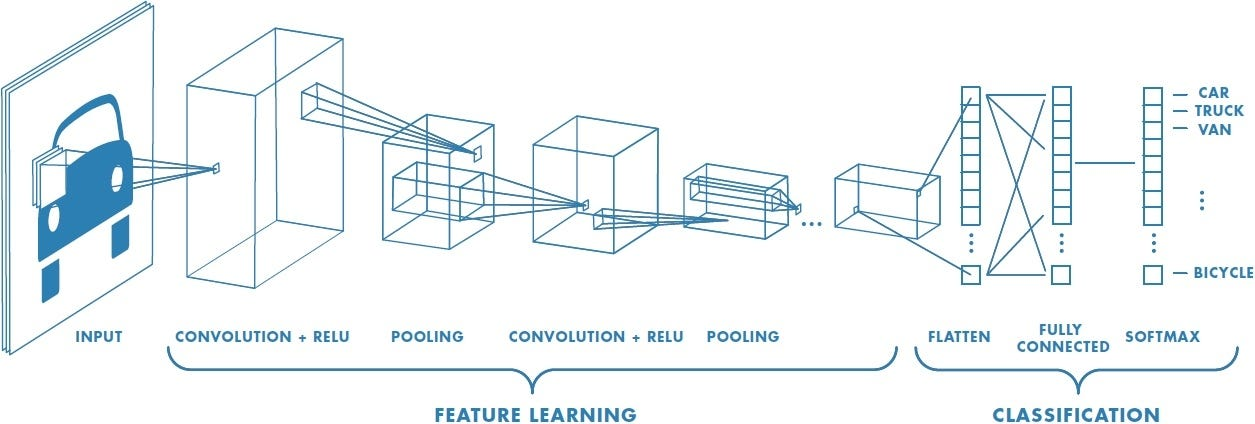
\includegraphics [width=\textwidth]{image/bab2/arsitektur-cnn.jpg}}
    \caption{Arsitektur CNN \citep{wardani2023klasifikasi}}
    \label{Arsitektur CNN}
\end{figure}

\par Pada Gambar \ref{Arsitektur CNN} dapat dilihat bahwa konvolusi merupakan langkah awal dalam pengolahan gambar yang digunakan untuk mengekstraksi fitur penting dari gambar \textit{input}. Dalam konvolusi, hubungan antar piksel dipertahankan dengan cara mengoperasikan kotak kecil pada masukan untuk memahami fitur-fitur gambar. Konvolusi melibatkan operasi matematika linear yang mencakup perkalian antara matriks gambar dan filter (\textit{kernel}) yang merupakan matriks bobot dua dimensi.

\par Fungsi dari lapisan \textit{pooling} adalah untuk secara bertahap mengurangi ukuran representasi spasial gambar, sehingga mengurangi jumlah parameter yang dibutuhkan dalam jaringan. Lapisan \textit{pooling} biasanya ditempatkan di antara lapisan-lapisan konvolusi. Lapisan ini beroperasi secara independen pada setiap peta fitur \citep{monedero2021cyber}.

\par CNN merupakan terobosan besar dalam pengenalan gambar. Mereka belajar langsung dari data gambar, menggunakan pola untuk mengklasifikasikan gambar dan menghilangkan kebutuhan ekstraksi fitur manual. Saat ini, CNN merupakan topik yang menarik dalam \textit{machine learning}, dan telah menunjukkan kinerja yang sangat baik dalam klasifikasi \citep{khan2020survey}. 



\section{\textit{Long Short Term Memory}}

\par \textit{Long Short Term Memory} (LSTM) adalah tipe dari \textit{Recurrent Neural Network} (RNN) yang diciptakan untuk menangani data yang bersifat \textit{sequential} seperti data \textit{time series, speech}, dan \textit{text}. LSTM ini dikembangkan untuk mengatasi masalah \textit{vanishing gradient} yang ada dalam RNN tradisional, yang membuatnya sulit bagi jaringan untuk mempelajari ketergantungan jangka panjang \citep{brownlee2017gentle}.

\par Menurut \citep{alom2019state} LSTM adalah model jaringan saraf yang menggunakan \textit{cell state} untuk menyimpan informasi dari \textit{input} sebelumnya. \textit{Cell state} memiliki tiga gerbang: \textit{input gate} ($i_t$), \textit{forget gate} ($f_t$), dan \textit{output gate} ($o_t$) yang bisa dilihat pada Gambar \ref{diagram_lstm}.

\begin{figure}[H]
\centering
{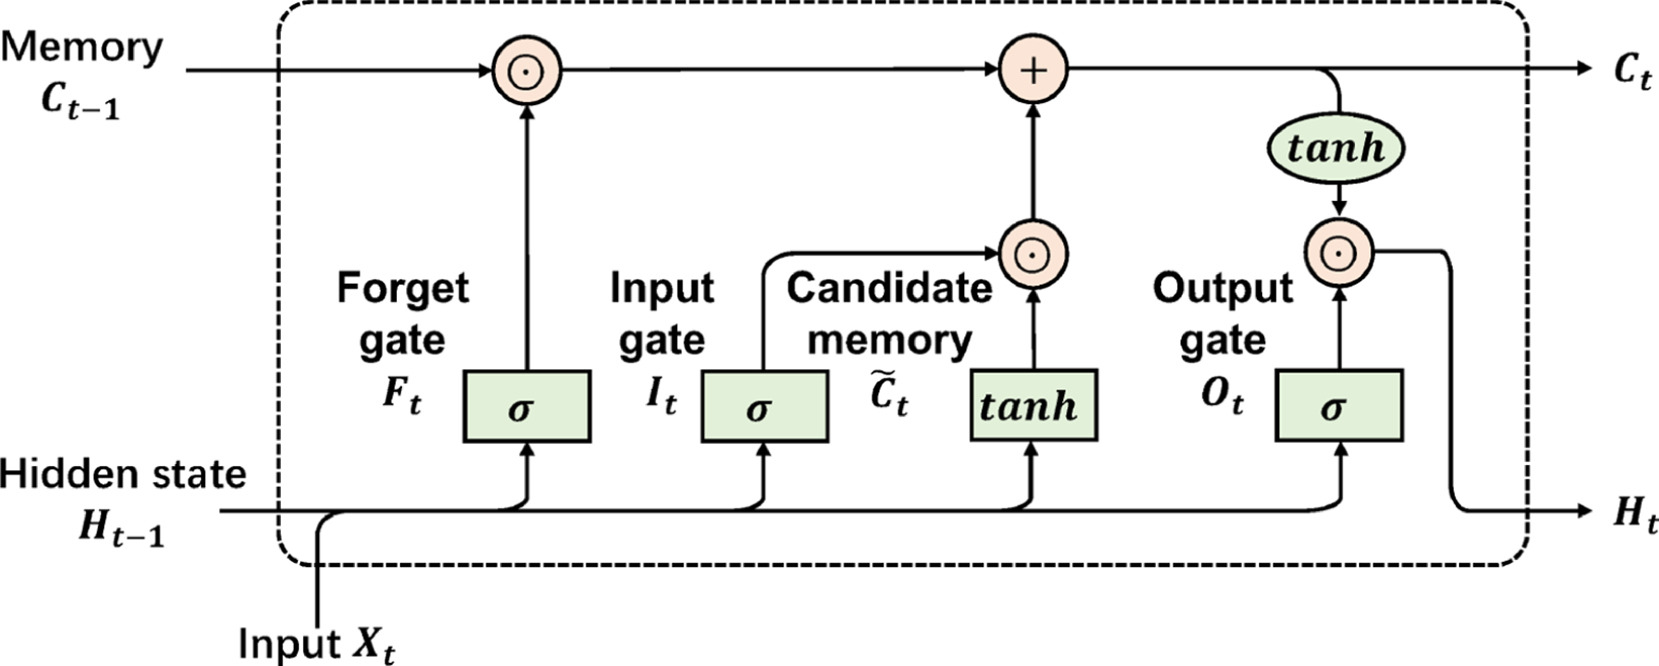
\includegraphics [width=\textwidth]{image/bab2/lstm-architecture.jpg}}
\caption{Arsitektur LSTM \citep{LUO2023107413}}
\label{diagram_lstm}
\end{figure}

\par \textit{Input gate} ($i_t$) digunakan untuk mengontrol pengaruh data yang masuk saat ini terhadap bobot unit tersebut, \textit{forget gate} ($f_t$) bertujuan untuk mengendalikan pengaruh riwayat informasi pada bobot unit saat ini, \textit{output gate} ($o_t$) bertujuan dalam mengendalikan ekspor nilai keadaan unit memori \citep{huang2021fault}.


% \section{\textit{Transformers}}

% \par \textit{Transformers} adalah jenis jaringan saraf yang dapat memproses data berurutan tanpa mengandalkan lapisan \textit{recurrent} dan \textit{convolution}. Pada \textit{transformers} mereka menggunakan mekanisme yang disebut \textit{attention}, yang memungkinkan mereka fokus pada bagian yang paling relevan dari \textit{input} dan \textit{output} pada setiap langkah. \textit{Attention} juga memungkinkan \textit{transformer} untuk menangkap ketergantungan jarak jauh dan informasi kontekstual, yang penting untuk \textit{Natural Language Processing} (NLP). Pada gambar \ref{fig: arsitektur transformer} dapat dilihat bahwa \textit{transformers} terdiri dari \textit{encoder} dan \textit{decoder}. \textit{Encoder} bertugas untuk mengubah teks \textit{input} menjadi urutan representasi tersembunyi, yang disebut \textit{embedding}. \textit{Decoder} bertugas untuk mengambil \textit{embedding} dan menghasilkan teks \textit{output}, satu token pada satu waktu. \textit{Encoder} dan \textit{decoder} terdiri dari beberapa lapisan yang terdiri dari dua sub-lapisan. Sub-lapisan pertama adalah \textit{multi-head self-attention layer}, dan sub-lapisan kedua adalah \textit{feed-forward neural network}. \textit{Multi-head self-attention layer} bertugas untuk mengambil representasi teks \textit{input} dan menghasilkan representasi teks \textit{output} yang lebih baik. \textit{Feed-forward neural network} bertugas untuk mengubah representasi teks \textit{output} menjadi representasi teks \textit{output} yang lebih baik \citep{vaswani2017attention}.

% \begin{figure}[H]
%     \centering
%     {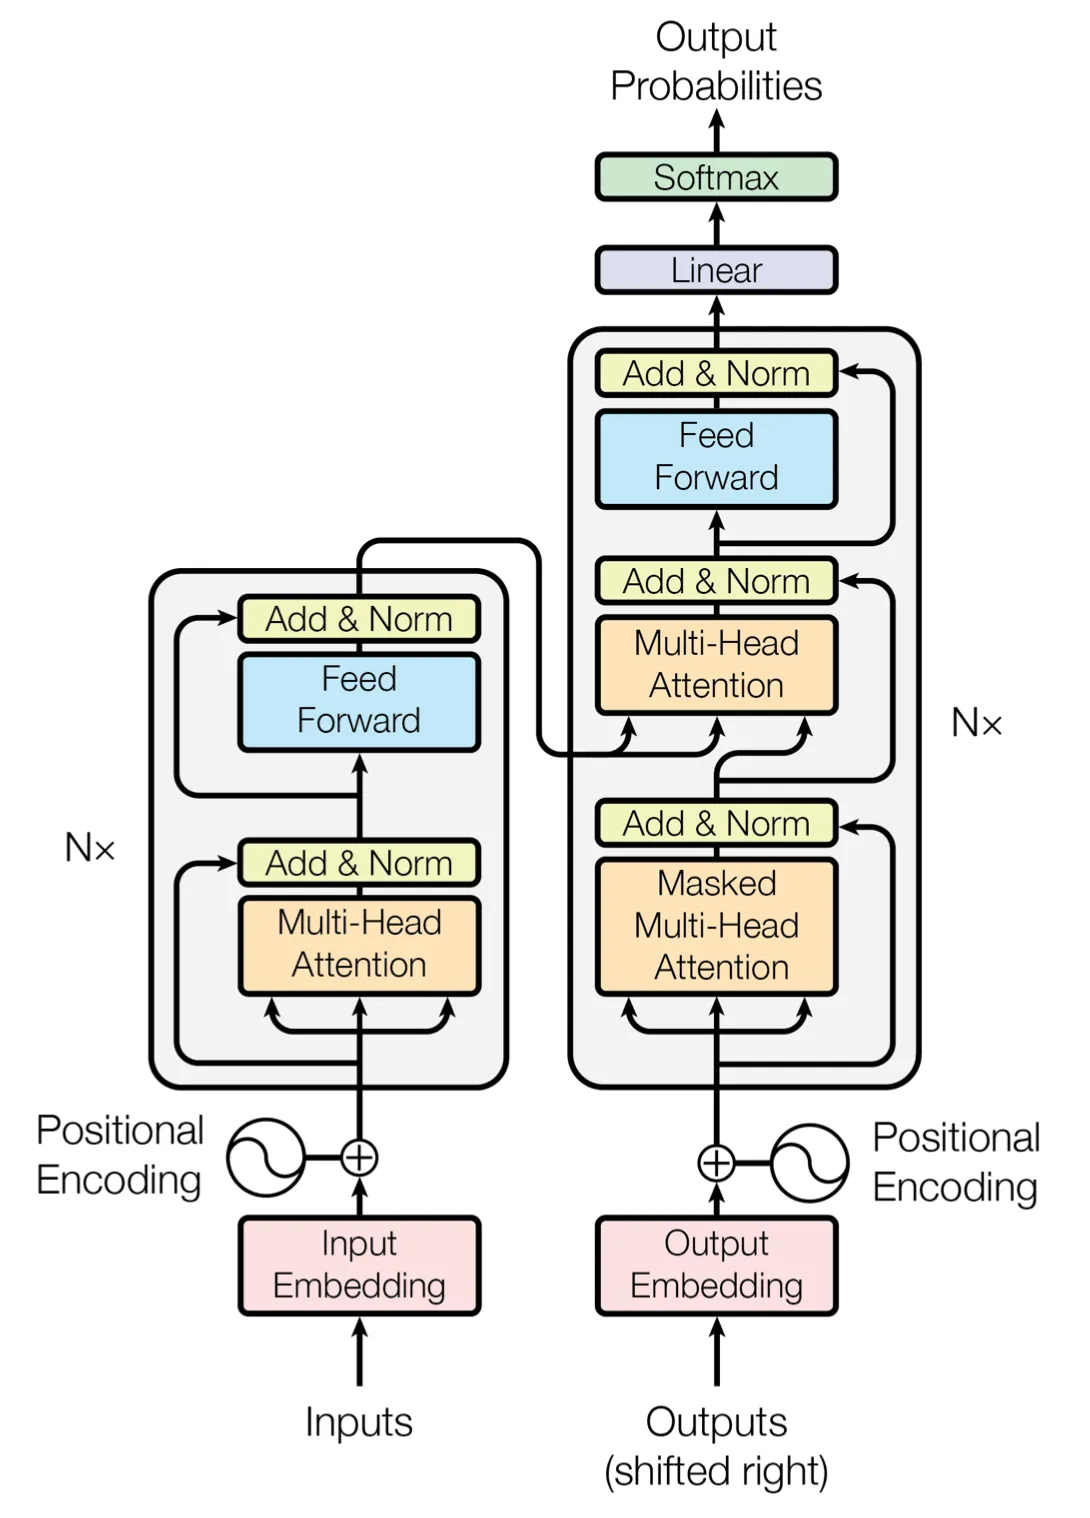
\includegraphics [width = 9cm, height= 15cm]{image/bab2/transformers.png}}
%     \caption{Arsitektur \textit{transformers} \citep{vaswani2017attention}}
%     \label{fig: arsitektur transformer}
% \end{figure}



% \subsection{\textit{Bidirectional Encoder Representation From Transformers} (BERT)}

% \par \textit{Bidirectional Encoder Representation From Transformers} (BERT) adalah 

% \subsection{\textit{Vision Transformer} (ViT)}

% \textit{Vision Transformer} (ViT) adalah model yang diciptakan untuk tugas \textit{computer vision}. Model ini menggunakan arsitektur \textit{transformer} untuk menangani tugas-tugas \textit{computer vision} seperti klasifikasi gambar, deteksi objek, dan segmentasi gambar. ViT mampu mengakses informasi global dan berinteraksi dengan elemen-elemen dalam gambar dengan baik, dan telah menunjukkan hasil yang tinggi dalam berbagai tugas \textit{computer vision}. \par Pada gambar \ref{fig: arsitektur vit} \citep{dosovitskiy2010image}.

% \begin{figure}[H]
%     \centering
%     {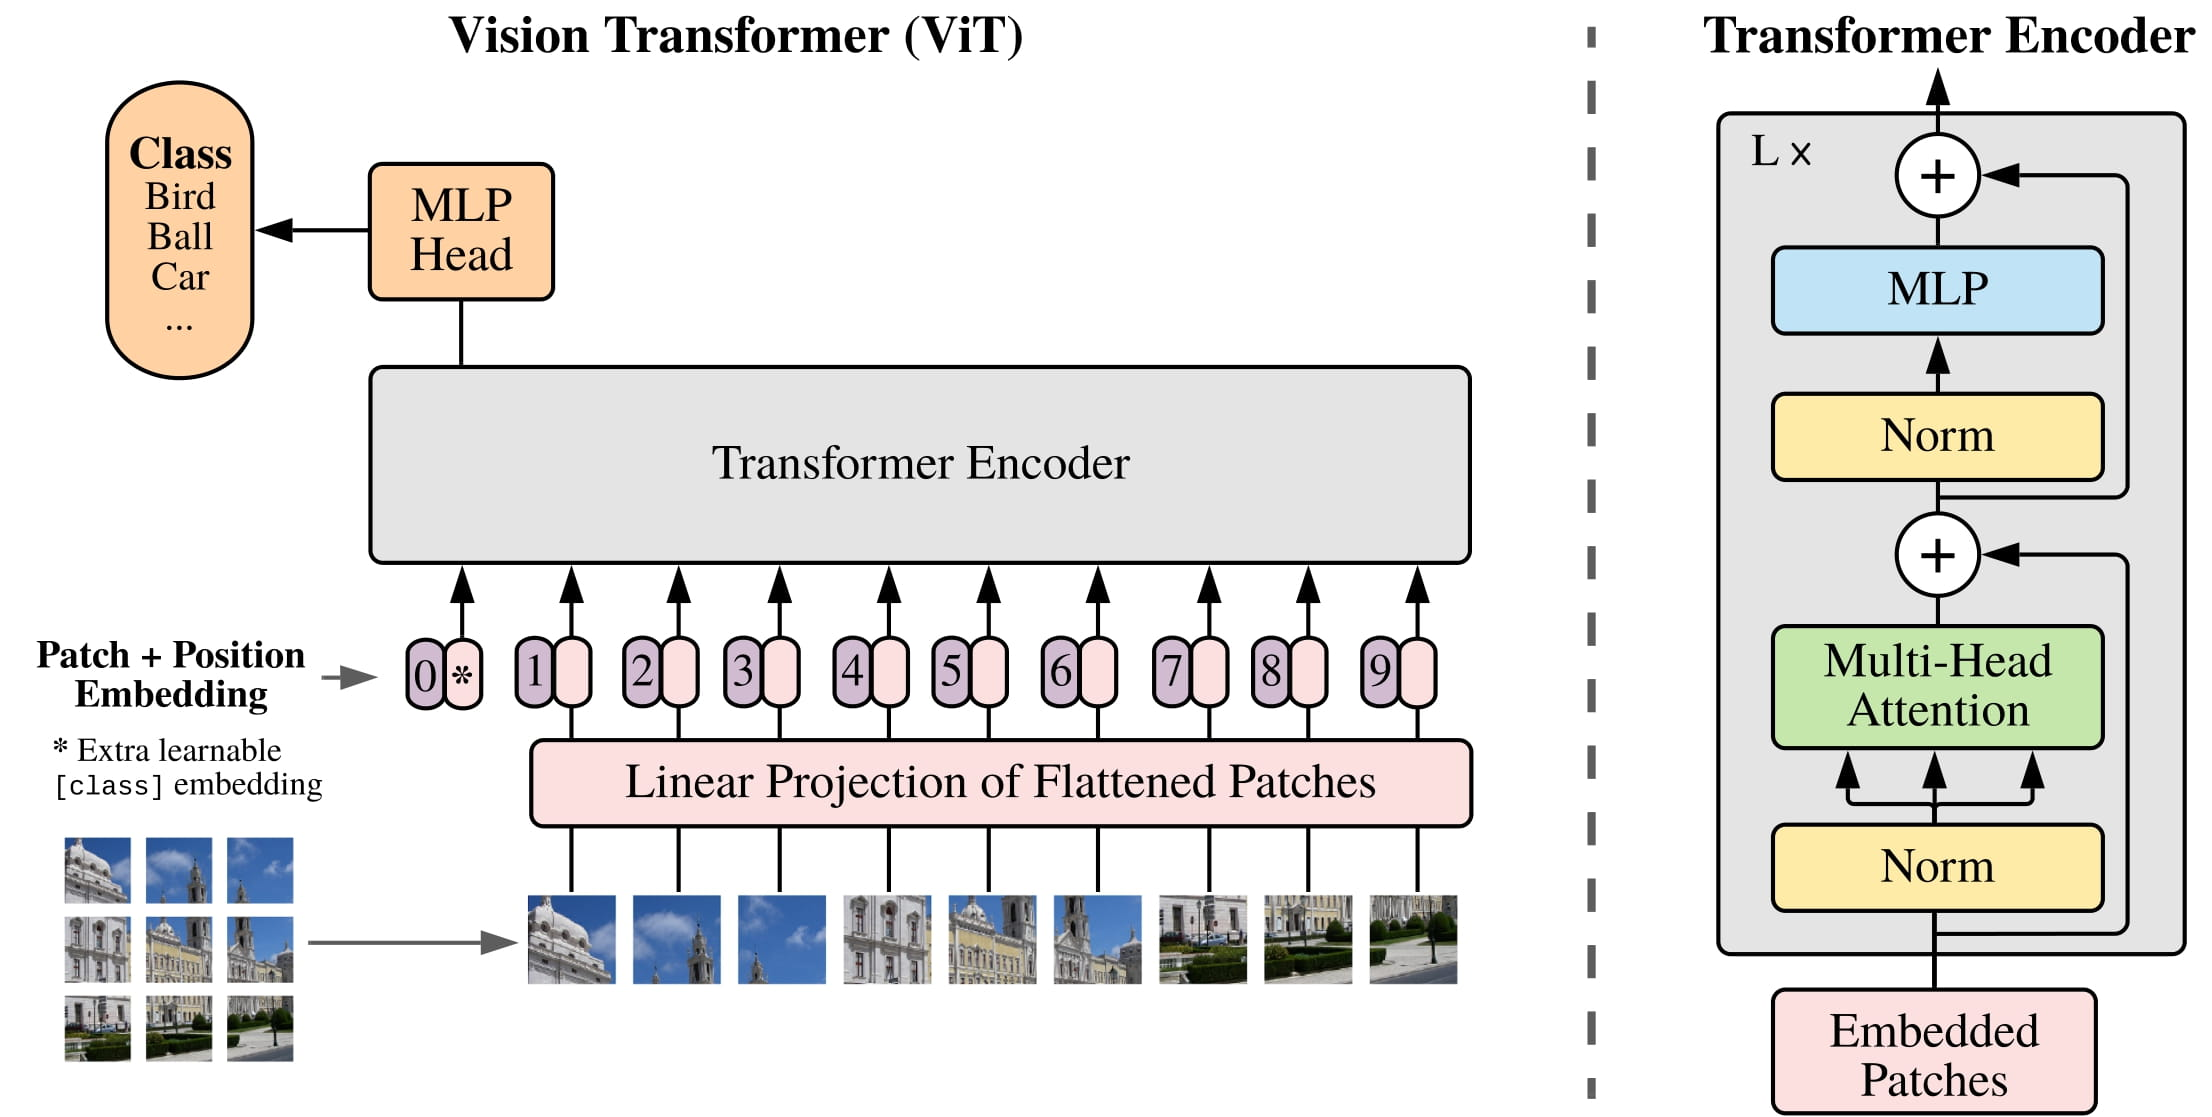
\includegraphics [width=\textwidth]{image/bab2/vit_architecture.jpg}}
%     \caption{Arsitektur ViT \citep{dosovitskiy2010image}}
%     \label{fig: arsitektur vit}
% \end{figure}







\section{\textit{Transfer Learning}}

\par \textit{Transfer learning} digunakan untuk meningkatkan pembelajaran dari satu domain dengan mentransfer informasi dari domain terkait. Kita dapat mengambil pengetahuan dunia nyata non-teknis untuk memahami mengapa \textit{transfer learning} memungkinkan. Pertimbangkan contoh dua orang yang ingin belajar bermain piano. Satu orang tidak memiliki pengalaman sebelumnya dalam bermain musik, dan orang lain memiliki pengetahuan musik yang luas melalui bermain gitar. Orang dengan latar belakang musik yang luas akan dapat belajar piano dengan lebih efisien dengan mentransfer pengetahuan musik yang sudah dipelajari sebelumnya ke tugas belajar bermain piano. Satu orang dapat mengambil informasi dari tugas yang sudah dipelajari sebelumnya dan menggunakannya secara bermanfaat untuk belajar tugas yang terkait \citep{pan2009survey}.


\par \textit{Transfer learning} pada \textit{Artificial Neural Network} (ANN) bisa dibayangkan seperti seseorang yang belajar menjadi lebih mudah, cepat, dan akurat dalam memahami tugas dan konsep baru jika mereka sudah memiliki pengalaman belajar yang serupa dengan konsep baru yang ingin dipelajari. Ini mirip dengan bagaimana seorang individu dapat lebih mudah memahami fisika setelah belajar matematika atau bagaimana seseorang dapat lebih lancar mengendarai truk setelah menguasai kemampuan mengemudi mobil. Pada dasarnya \textit{transfer learning} terjadi ketika pemahaman tentang suatu konteks dipengaruhi oleh pemahaman sebelumnya tentang konteks yang mirip \citep{cirecsan2012transfer}. Intinya adalah bahwa \textit{transfer learning} memungkinkan kita untuk menggunakan pengetahuan yang sudah ada untuk memecahkan masalah baru seperti yang ditunjukkan pada Gambar \ref{transfer_learning}.

\begin{figure}[H]
\centering
{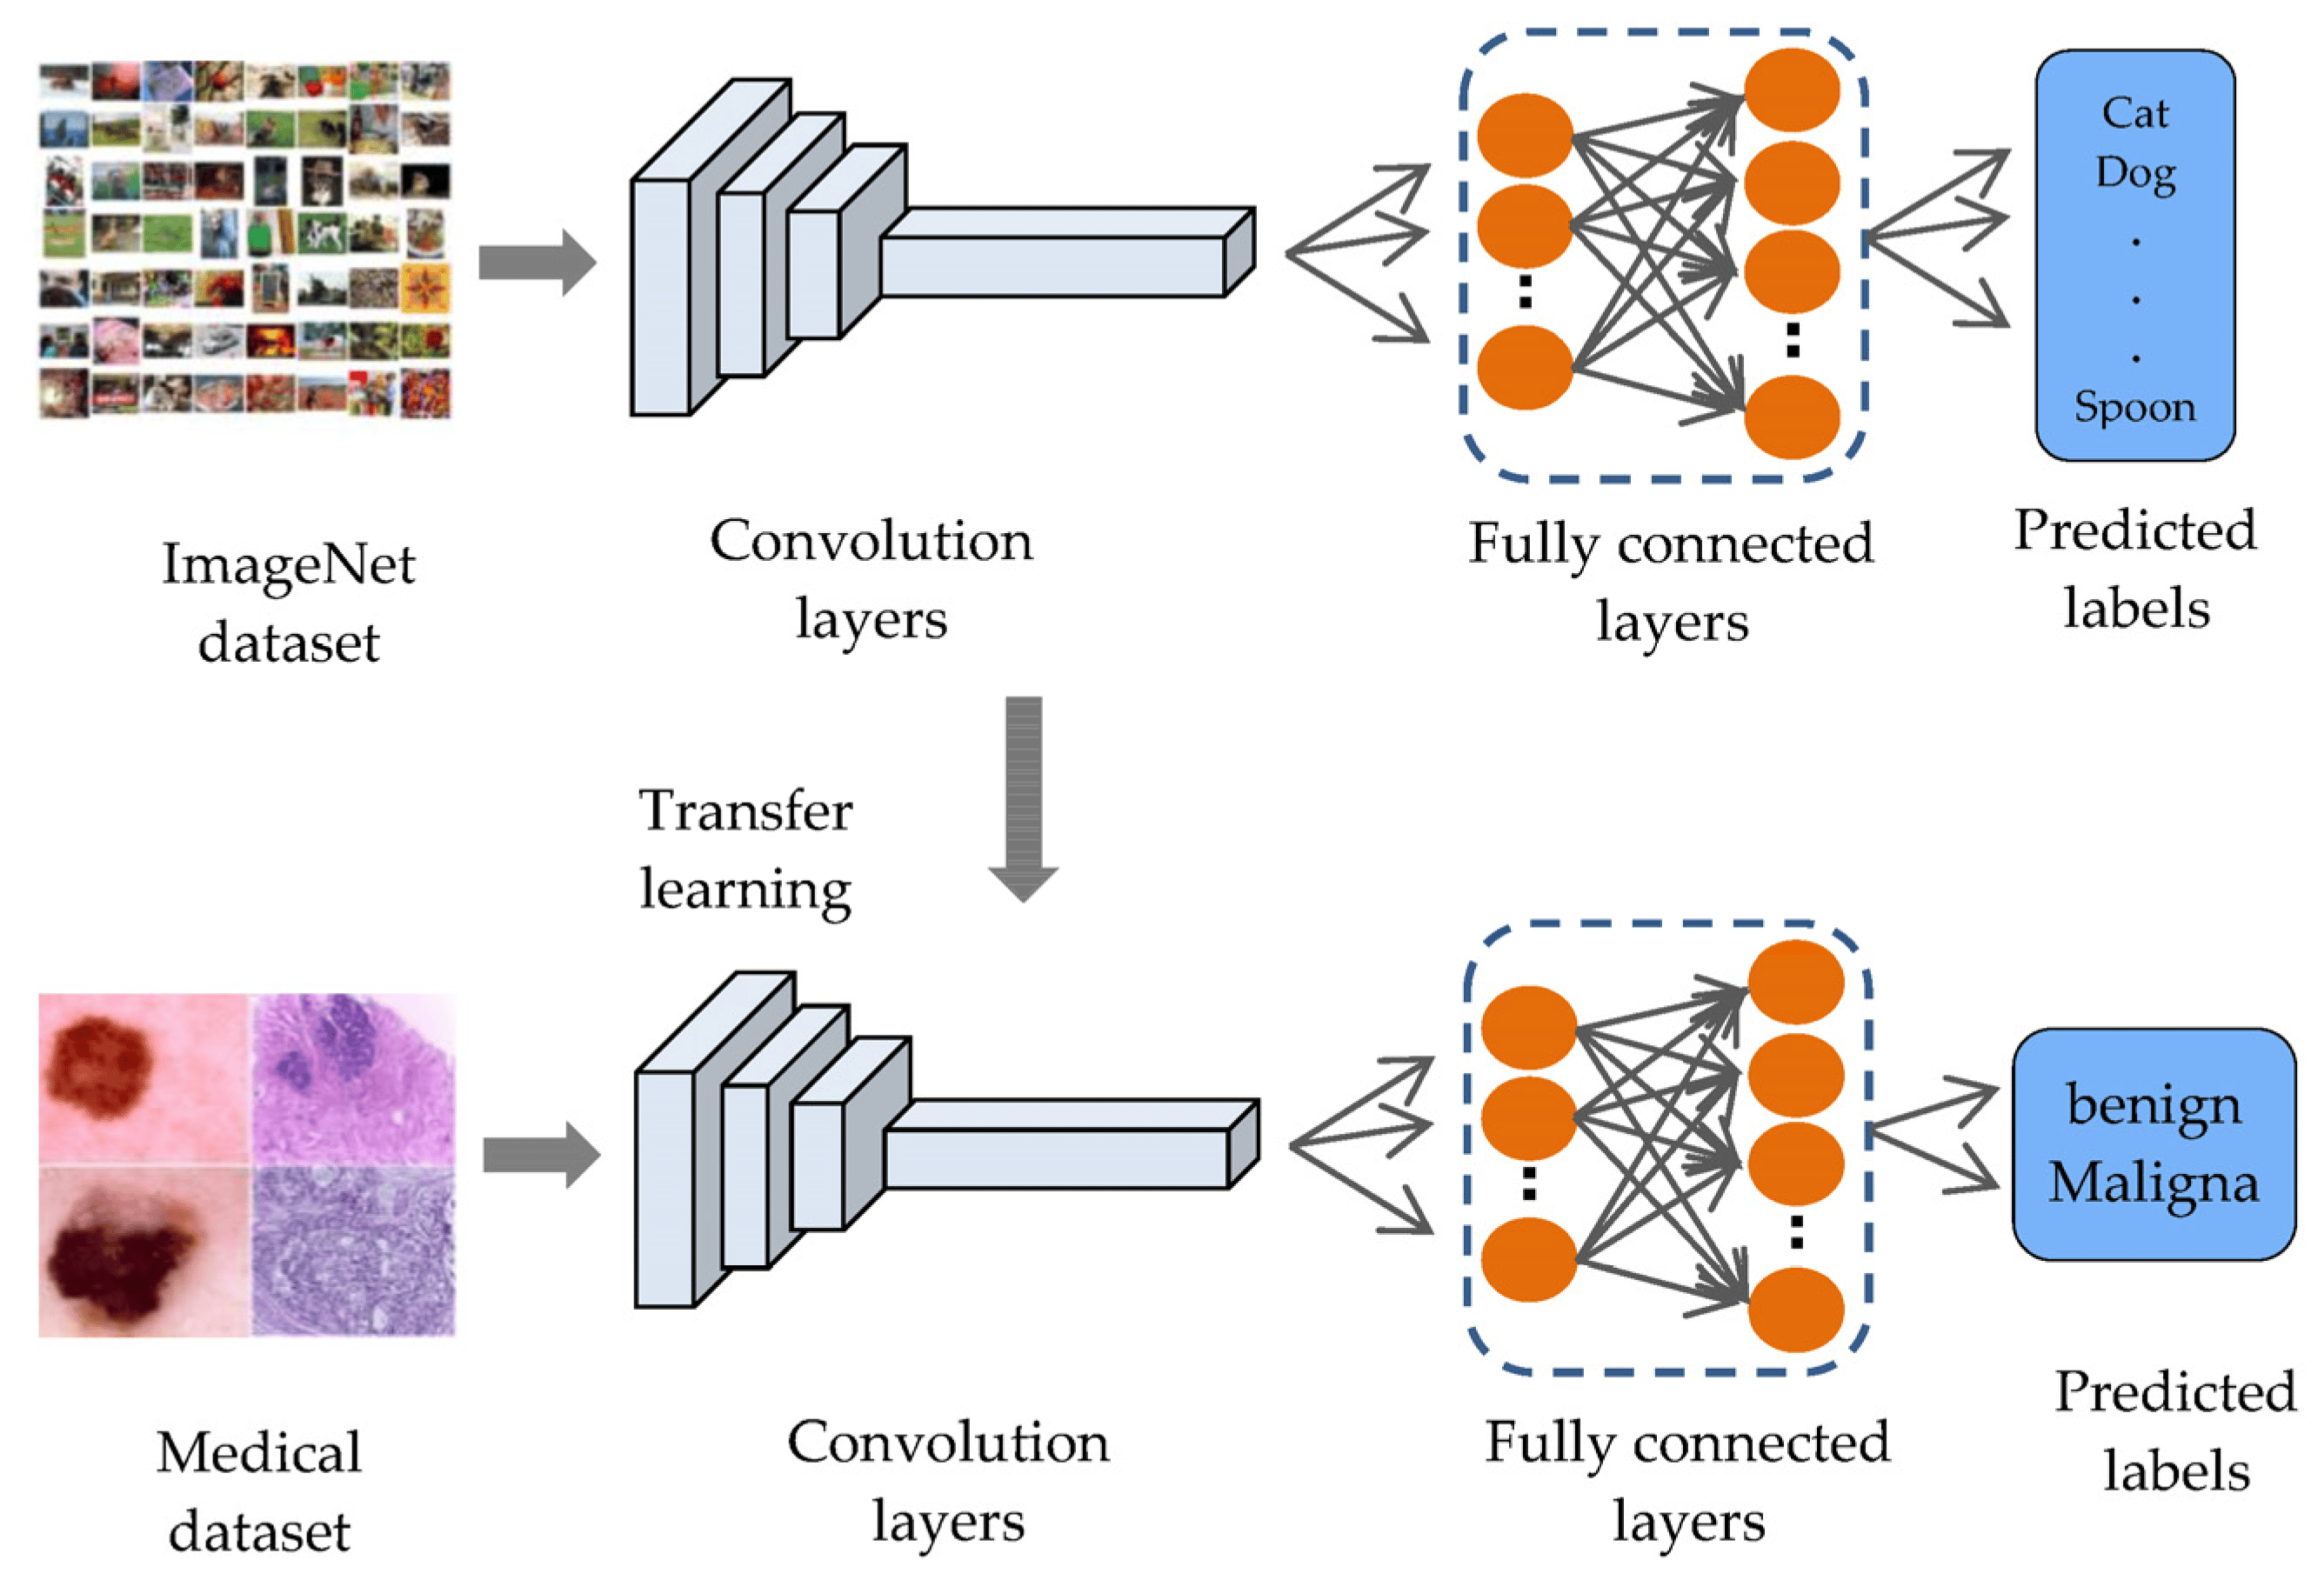
\includegraphics [width = 14cm, height= 8cm]{image/bab2/transfer-learning.png}}
\caption{Konsep penggunaan \textit{transfer learning} \citep{mukhlif2023incorporating}}
\label{transfer_learning}
\end{figure}

\par Model dasar yang digunakan dalam \textit{transfer learning} adalah \textit{pre-trained} model, dimana bobot di seluruh jaringan saraf tiruan sudah disesuaikan untuk data tertentu. Ini memungkinkan model untuk memiliki pemahaman yang lebih mendalam tentang fitur dasar dan fitur tingkat tinggi yang dapat mempercepat proses pelatihan. Secara konsisten, model jaringan saraf yang telah dilatih sebelumnya memberikan hasil prediksi yang lebih tepat dibandingkan dengan jaringan saraf yang dimulai dengan bobot-bobot yang diinisiasi secara acak dalam konteks masalah yang melibatkan data yang sudah memiliki label \citep{cirecsan2012transfer}.


\par VGG19 merupakan salah satu model \textit{pre-trained} yang digunakan dalam penelitian ini. VGG19 adalah model CNN yang memiliki 19 lapisan. Model ini dilatih pada \textit{dataset} ImageNet yang memiliki 1000 kelas dan 1,2 juta gambar. Model ini memiliki 16 lapisan konvolusi dan 3 lapisan \textit{fully connected}. Model ini memiliki 138 juta parameter dan 20 miliar operasi \citep{simonyan2014very}. Arsitektur VGG19 dapat dilihat pada Gambar \ref{Arsitektur VGG19}.


\begin{figure}[H]
    \centering
    {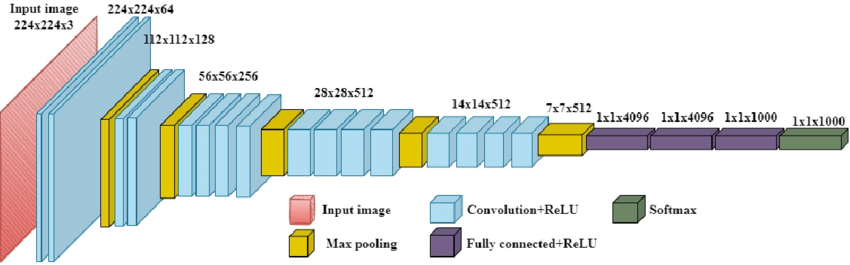
\includegraphics [width=\textwidth]{image/bab2/vgg19.jpeg}}
    \caption{Arsitektur VGG19 \citep{nguyen2022vgg} }
    \label{Arsitektur VGG19}
\end{figure}

\par \textit{Bootstrapping Language-Image Pre-training for Unified Vision-Language Understanding and Generation} (BLIP) adalah sebuah kerangka dari \textit{Vision Language Pre-Training} (VLP). BLIP mampu melakukan berbagai tugas \textit{multimodal} seperti \textit{Visual Question Answering} (VQA), \textit{image captioning}, dan lain-lain. Dalam hal ini, BLIP mengusulkan sebuah model \textit{multimodal mixture of encoder-decoder} yang dapat beroperasi secara fleksibel sebagai \textit{encoder} dan \textit{decoder} untuk berbagai tugas penglihatan bahasa. BLIP mampu memajukan \textit{pre-training} terunifikasi untuk transfer pembelajaran lintas tugas \textit{vision-language}. Berikut ini dapat dilihat arsitektur pada BLIP pada Gambar \ref{Arsitektur BLIP}.

\begin{figure}[H]
    \centering
    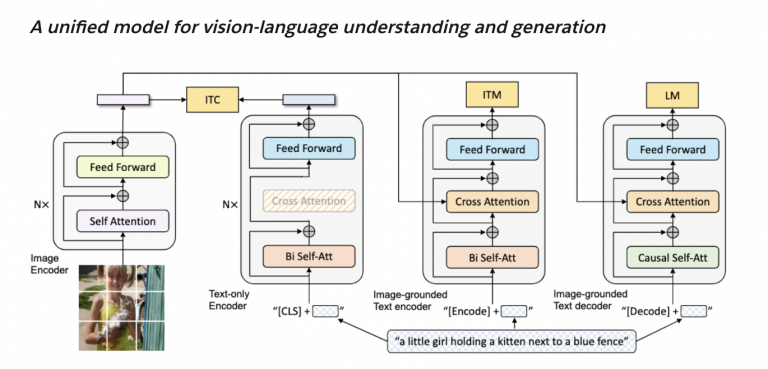
\includegraphics[width=\textwidth]{image/bab2/arsitektur-blip.png}
    \caption{Arsitektur BLIP \citep{li2022blip}}
    \label{Arsitektur BLIP}
\end{figure}

\par BLIP memiliki tiga fungsionalitas yang dapat dilihat sebagai berikut:

\begin{enumerate}

    \item{\textit{Unimodal encoder} yang memisahkan proses \textit{encode} gambar dan teks. \textit{Image encoder} didasarkan pada \textit{Vision Transformer} (ViT), sementara \textit{encoder} teks mirip dengan \textit{Bidirectional Encoder Representation from Transformer} (BERT). Disini, terdapat token khusus [CLS] yang ditambahkan di awal \textit{input} teks untuk merangkum kalimat.}

    \item{\textit{Image-grounded text encoder} yang bertujuan memasukkan informasi visual ke dalam \textit{encoder} teks. Pada bagian ini dilakukan dengan menyisipkan lapisan \textit{cross-attention} antara lapisan \textit{self-attention} dan jaringan \textit{feed-forward} untuk setiap blok transformer dari \textit{encoder} teks. Pada bagian ini terdapat token khusus yaitu [Encode] yang ditambahkan ke teks, dan \textit{embedding output} dari [Encode] ini digunakan sebagai representasi multimodal dari pasangan gambar dan teks.}

    \item{\textit{Image grounded text decoder} memodifikasi \textit{encoder} teks dengan menggantikan lapisan \textit{bidirectional self-attention} dengan lapisan \textit{causal self-attention}. Di bagian ini, token khusus [Decode] digunakan untuk menandai awal dari sebuah urutan.}

\end{enumerate}

\par Pada gambar \ref{Arsitektur BLIP} dijelaskan tiga tujuan dari arsitektur BLIP. Penjelasan tiga tujuan BLIP dapat dilihat sebagai berikut:

\begin{enumerate}
    \item{\textit{Image-Text Contrastive Loss} (ITC) bertujuan mengaktifkan \textit{unimodal encoder}. ITC mendorong keselarasan dalam ruang fitur transformer visual dan transformer teks dengan memastikan pasangan gambar dan teks yang positif memiliki representasi yang mirip dibandingkan dengan pasangan negatif.}

    \item{\textit{Image-Text Matching Loss} (ITM) bertujuan dalam mengaktifkan \textit{encoder} teks berdasarkan gambar. Bagian ini merupakan tugas klasifikasi biner dimana model memprediksi apakah pasangan gambar dan teks cocok atau tidak cocok berdasarkan fitur \textit{multimodal} mereka.}

    \item{\textit{Language Modelling Loss} (LM) bertujuan mengaktifkan \textit{decoder} teks berdasarkan gambar. Ini berfokus menghasilkan deskripsi teks yang dikondisikan pada gambar yang diberikan.}


\end{enumerate}

\par Intinya, BLIP menggunakan model serbaguna yang dapat menyatukan informasi visual ke dalam pemrosesan teks. Selama tahap pra-pelatihan, BLIP secara simultan mengoptimalkan tujuan keselarasan representasi visual dan teks, pencocokan pasangan gambar dan teks, serta pembangkitan deskripsi dalam bahasa dan gambar \citep{li2022blip}.

% \par ViLT (\textit{Vision-and-Language Transformer}) adalah suatu struktur model yang menggabungkan informasi dari unsur visual dan teks untuk berbagai tugas yang melibatkan unsur visual dan bahasa, seperti penggantian keterangan gambar (\textit{image captioning}), menjawab pertanyaan visual (\textit{visual question answering}), dan lain-lain. ViLT merupakan perkembangan lebih lanjut dari model VLP (\textit{Vision and Language Pre-training}) dan diciptakan dengan tujuan untuk mengatasi beberapa masalah yang ada pada model VPL sebelumnya. Keunggulan dari model ViLT terletak pada kemampuannya yang lebih baik dibandingkan dengan model VLP, yang disebabkan oleh pendekatan yang lebih sederhana dan efisien dalam memproses informasi visual masukan, berbeda dengan model VPL yang memerlukan ekstraksi fitur gambar yang kompleks, seperti deteksi objek dan arsitektur konvolusi. Arsitektur ViLT mengurangi ketergantungan pada ekstraksi fitur gambar yang rumit dan mengusulkan suatu pendekatan yang lebih langsung dalam memproses informasi visual masukan, sehingga menghasilkan kecepatan yang lebih tinggi, tetapi tetap mempertahankan atau meningkatkan kinerja dalam tugas-tugas turunan yang melibatkan unsur visual dan bahasa \citep{kim2021vilt}. Struktur arsitektur ViLT dapat dilihat pada gambar \ref{Arsitektur ViLT}.

% \begin{figure}[H]
%     \centering
%     {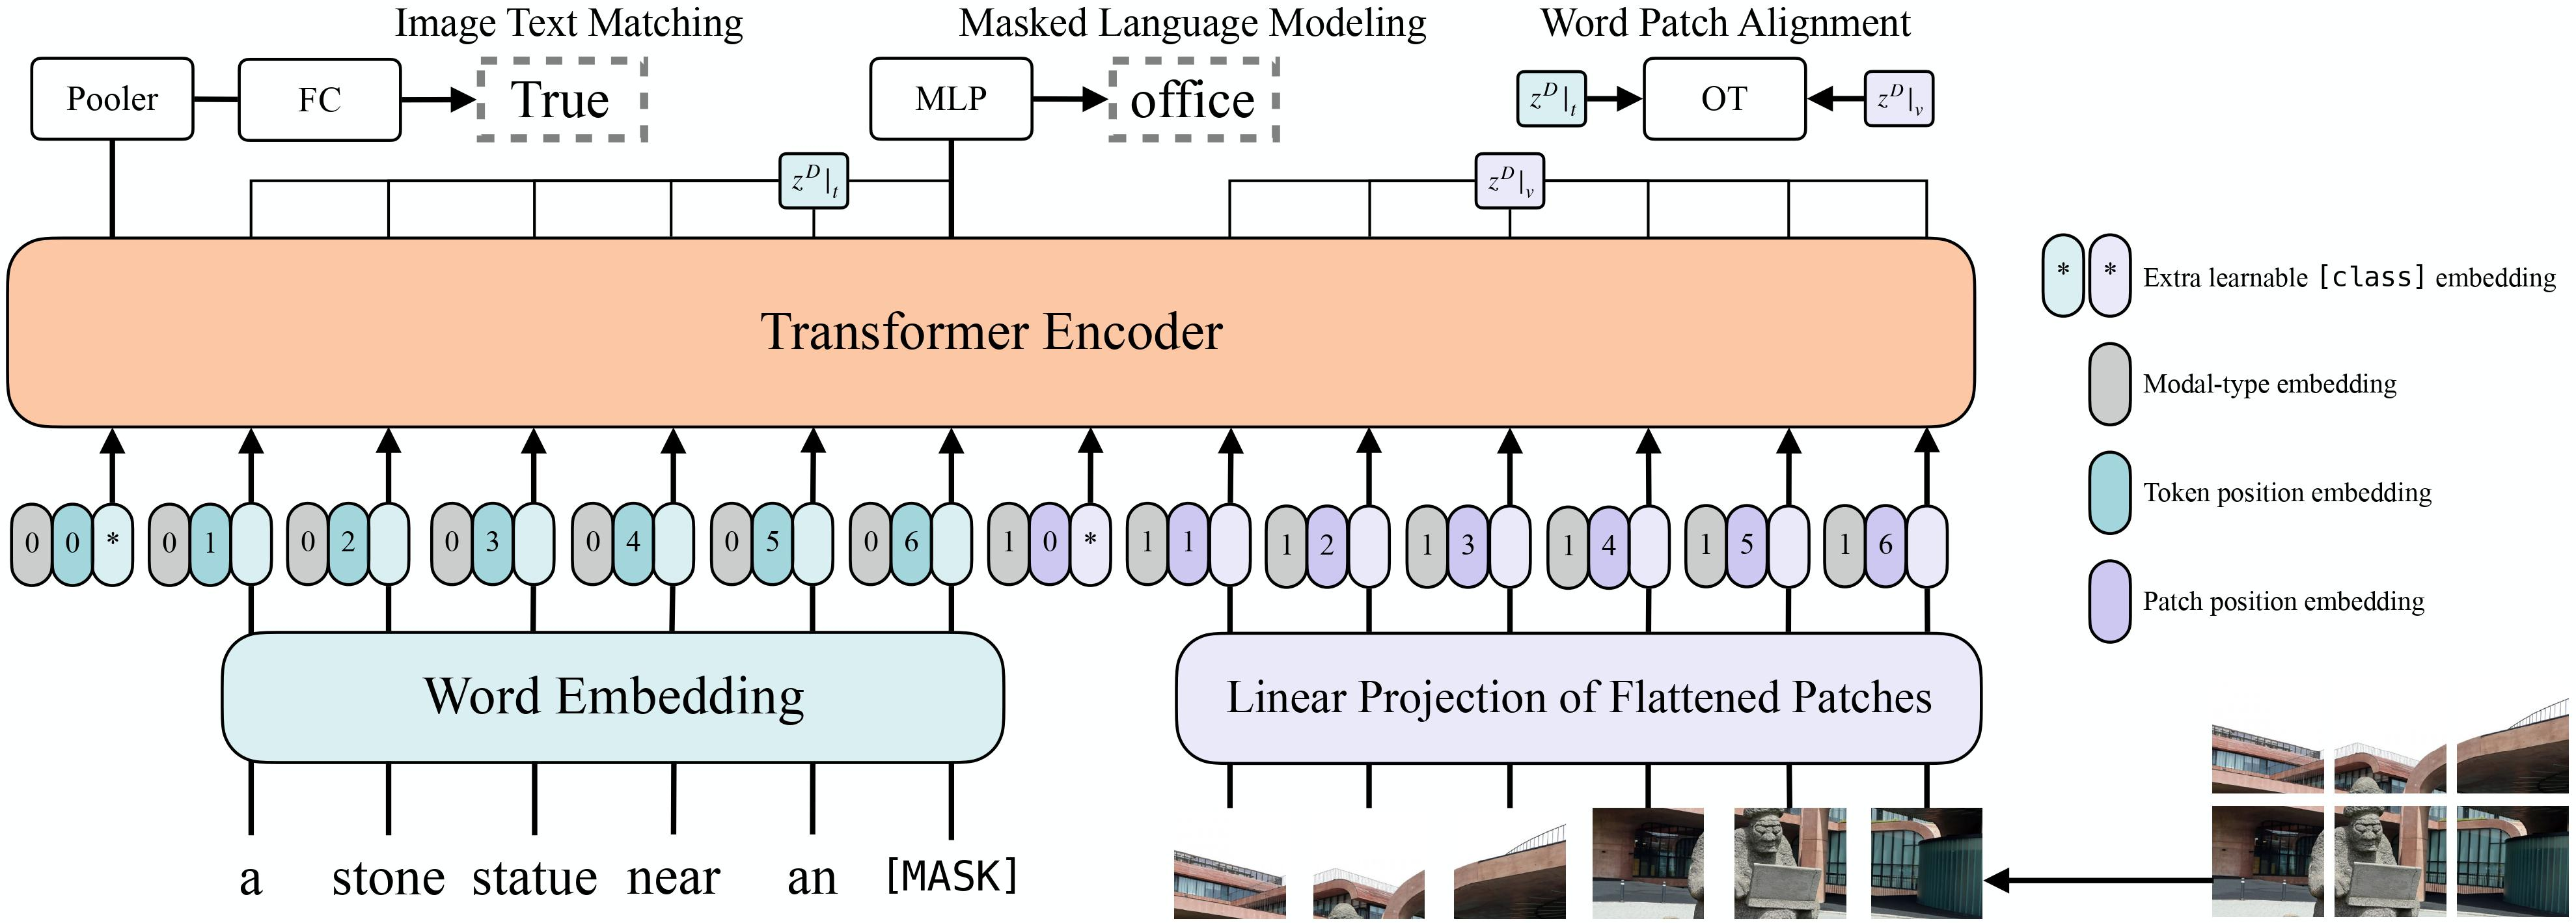
\includegraphics [width = 15cm, height= 6cm]{image/bab2/vilt_architecture.jpg}}
%     \caption{Arsitektur ViLT \citep{kim2021vilt} }
%     \label{Arsitektur ViLT}
% \end{figure}


\section{Matriks Evaluasi}

\par Matriks evaluasi yang digunakan dalam menilai kinerja model \textit{medical} VQA dapat dikategorikan menjadi dua jenis, yaitu \textit{classification-based metrics} dan \textit{language-based metrics}. Pada umumnya metrik yang digunakan pada kasus klasifikasi, seperti akurasi dan \textit{F1-score}. Metrik ini memperlakukan jawaban sebagai hasil dari klasifikasi dan menghitung pencocokan yang tepat untuk akurasi, presisi, \textit{recall} dan lain-lain. Sedangkan metrik yang digunakan pada kasus \textit{language-based} bertujuan untuk mengevaluasi tugas seperti penerjemah, \textit{image captioning}, VQA, dan lain-lain. \textit{Dataset} seperti VQA-Med-2018, VQA-Med-2019, PathVQA, VQA-Med-2020, dan VQA-Med-2021 menggunakan metrik \textit{language-based} seperti \textit{BLEU}, untuk mengevaluasi kinerjanya \citep{lin2023medical}.

\par \textit{Confusion matrix} adalah suatu alat pengukuran kinerja yang digunakan dalam konteks masalah klasifikasi pada pembelajaran mesin. Matriks ini terdiri dari tabel memberikan gambaran visual dan ringkasan mengenai kinerja algoritma klasifikasi. Tiap baris dalam matriks mencerminkan contoh dalam kelas aktual, sementara setiap kolom mencerminkan contoh dalam kelas yang diprediksi. \textit{Confusion matrix} sangat bermanfaat untuk menilai efektivitas suatu model, terutama ketika terdapat ketidakseimbangan jumlah observasi antar kelas atau ketika menghadapi lebih dari dua kelas dalam suatu \textit{dataset}. \textit{Confusion matrix} merefleksikan nilai \textit{True Positive} (TP) yang menunjukkan klasifikasi yang tepat pada kelas yang relevan, nilai \textit{False Positive} (FP) yang mencerminkan klasifikasi di kelas yang seharusnya tidak relevan, nilai \textit{False Negative} (FN) yang menunjukkan klasifikasi di kelas yang salah ketika seharusnya relevan, dan nilai \textit{True Negative} (TN) yang mencerminkan klasifikasi yang benar di kelas yang tidak relevan. Gambar \textit{confusion matrix} dapat dilihat pada Gambar \ref{Confusion Matrix} \citep{KULKARNI202083}.

\begin{figure}[H]
    \centering
    {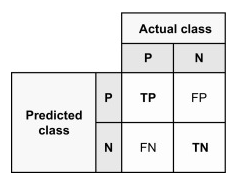
\includegraphics [width = 8cm, height= 5cm]{image/bab2/conf-matrix.png}}
    \caption{\textit{Confusion matrix} \citep{KULKARNI202083}}
    \label{Confusion Matrix}
\end{figure}

\subsection{Akurasi}

\par Pada umumnya akurasi adalah metrik yang mengukur perbandingan antara jumlah prediksi yang benar dengan jumlah total kasus yang dievaluasi \citep{hossin2015review}. Pada persamaan \ref{rumus-accuracy} menunjukkan bahwa rumus dari akurasi adalah jumlah prediksi yang benar dibagi dengan total prediksi yang dilakukan.

% Rumus Accuracy
\begin{equation}
    % rumus accuracy
    Akurasi = \frac{TP + TN}{TP + TN + FP + FN}
    \label{rumus-accuracy}
\end{equation}

% keterangan rumus accuracy
\begin{itemize}
    \item TP (\textit{True Positive}) adalah jumlah prediksi yang benar positif.
    \item TN (\textit{True Negative}) adalah jumlah prediksi yang benar negatif.
    \item FP (\textit{False Positive}) adalah jumlah prediksi yang salah positif.
    \item FN (\textit{False Negative}) adalah jumlah prediksi yang salah negatif.

\end{itemize}

\subsection{\textit{Bilingual Evaluation Understudy}}

\par \textit{Bilingual Evaluation Understudy} (BLEU) adalah metrik yang digunakan untuk mengukur kesamaan pada frase (n-grams) antara dua kalimat. BLEU adalah metrik original untuk penerjemah mesin dan juga bisa digunakan untuk tugas seperti pembuatan laporan medis \citep{li2021ffa}.

\par BLEU adalah metrik yang digunakan untuk mengevaluasi kualitas sistem terjemahan mesin \citep{papineni2002bleu}. Ini mengukur kemiripan antara terjemahan yang dihasilkan oleh mesin dan satu atau lebih referensi terjemahan menggunakan metrik presisi yang dimodifikasi dan hukuman singkat yang dimodifikasi dan \textit{brevity penalty} yang dimodifikasi.

\begin{equation}
    \text{BLEU} = \text{BP} \times \exp\left(\sum_{n=1}^{N} w_n \log p_n\right) 
    \label{rumus-bleu}
\end{equation}


% keterangan rumus BLEU

\begin{itemize}
    \item $BP$ adalah \textit{brevity penalty}.
    \item $N$ adalah jumlah maksimal n-gram.
    \item $w_n$ adalah bobot untuk n-gram.
    \item $p_n$ adalah presisi n-gram.

\end{itemize}

\par Berdasarkan persamaan \ref{rumus-bleu} \textit{Brevity Penalty} (BP)  menghukum jawaban singkat, $w_n$ adalah bobot antara 0 dan 1 untuk $\log p_n$ dan $\sum_{n=1}^{N} w_n = 1$, $p_n$ adalah nilai rata-rata geometris dari presisi n-gram yang dimodifikasi, dan N adalah panjang maksimum n-gram.

\par BLEU memiliki beberapa variasi, seperti BLEU-1, BLEU-2, BLEU-3, dan seterusnya. Variasi ini menunjukkan jumlah n-gram yang digunakan dalam perhitungan BLEU. Semakin tinggi nilai BLEU, semakin baik kualitas terjemahan mesin tersebut. Nilai BLEU berkisar dari 0 hingga 100, di mana 100 menunjukkan terjemahan yang sempurna. Berikut adalah penjelasan mengenai berbagai variasi BLEU:

\begin{enumerate}

    \item BLEU-1 adalah variasi dasar dari metrik BLEU yang hanya mempertimbangkan \textit{unigram} (kata tunggal). Perhitungan BLEU-1 mengukur seberapa baik kata-kata dalam hasil terjemahan sesuai dengan kata-kata dalam kalimat referensi tanpa mempertimbangkan urutan kata.

    \item BLEU-2 memperluas perhitungan dengan menggunakan \textit{bigram} (pasangan kata). Dalam BLEU-2, selain mempertimbangkan kesesuaian \textit{unigram}, juga diperiksa kesesuaian pasangan kata dalam hasil terjemahan dan kalimat referensi. Hal ini memberikan evaluasi yang lebih baik terhadap struktur kalimat terjemahan.

    \item BLEU-3 melangkah lebih jauh dengan menggunakan \textit{trigram} (tiga kata berturut-turut). Disini, evaluasi BLEU-3 memperhitungkan kesesuaian \textit{trigram} antara hasil terjemahan dan kalimat referensi. Semakin panjang n-gram yang digunakan, semakin ketat evaluasi terhadap kualitas terjemahan, karena memperhatikan konteks yang lebih luas dalam kalimat.

\end{enumerate}

\par Kesimpulannya, variasi-variasi ini menunjukkan bahwa dengan meningkatnya nilai "n" dalam n-gram, evaluasi terhadap terjemahan mesin menjadi lebih komprehensif dan memperhitungkan konteks yang lebih luas dalam kalimat \citep{papineni2002bleu}.






\par Deskripsi BLEU berbeda tergantung pada rentang nilai yang ada. Detail deskripsi untuk masing-masing rentang nilai BLEU dapat ditemukan di Tabel \ref{tabel-bleu} \citep{lavie2010evaluating}.

\begin{table}[H]
    \centering
    \caption{Deskripsi dari masing-masing nilai BLEU}
    \label{tabel-bleu}
    \begin{tabular}{|l|l|}
    \hline
    \textbf{Nilai BLEU} & \textbf{Deskripsi}                                                    \\ \hline
    \textless\ 10       & Hampir tidak dapat dipahami                                           \\ \hline
    10 - 19             & Sulit untuk mendapatkan intisari kalimat                              \\ \hline
    20 - 29             & Inti kalimat jelas, tetapi memiliki banyak kesalahan pada tata bahasa \\ \hline
    30 - 39             & Dapat dimengerti sebagai penerjemah kalimat yang baik                 \\ \hline
    40 - 49             & Terjemahan kalimat berkualitas tinggi                                 \\ \hline
    50 - 59             & Terjemahan kalimat sangat berkualitas dan memadai                     \\ \hline
    \textgreater\ 60    & Kemampuan menerjemah sering lebih bagus dari manusia                  \\ \hline
    \end{tabular}
\end{table}


\section{\textit{Visual Question Answering}}

\par \textit{Visual Question Answering} (VQA) adalah suatu tugas tentang bagaimana menjawab pertanyaan bebas pada sebuah gambar. Karena membutuhkan pemahaman bahasa yang mendalam tentang pertanyaan dan kemampuan untuk mengaitkannya dengan berbagai objek yang ada dalam gambar. Ini adalah tugas yang ambisius dan memerlukan teknik dari baik \textit{computer vision} dan \textit{natural language processing} \citep{hildebrandt2020scene}.

\par Salah satu contoh percobaan yang dilakukan oleh \citep{antol2015vqa}, mereka menerapkan \textit{baseline} \textit{Vanilla} VQA model yang dimana sebagai tolak ukur untuk metode \textit{deep learning}. Model ini menggunakan CNN untuk ekstraksi fitur dan jaringan LSTM atau \textit{recurrent network} untuk pemrosesan bahasa. Fitur-fitur ini digabungkan menggunakan suatu operasi untuk membentuk satu fitur bersama, yang digunakan untuk mengklasifikasikan salah satu jawaban seperti yang ditunjukkan dalam Gambar \ref{exp: visual question answering}.

\begin{figure}[H]
    \centering
    {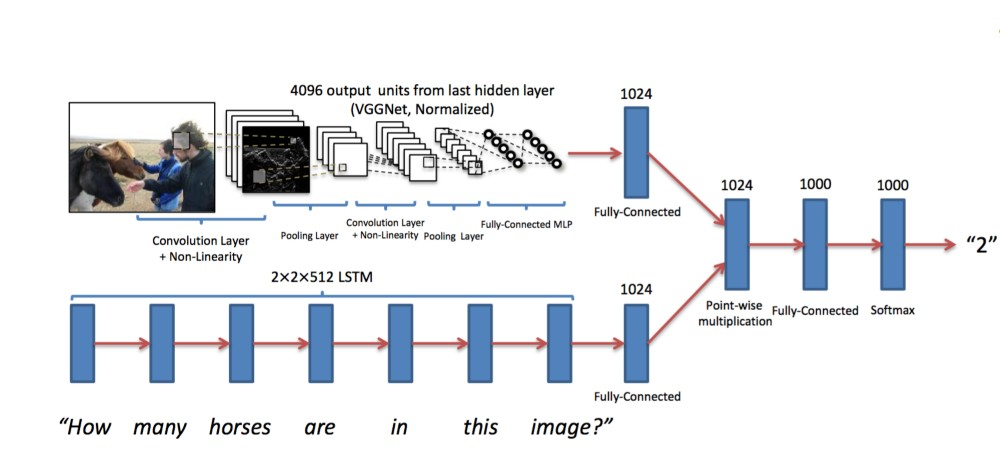
\includegraphics [width=\textwidth]{image/bab2/vqa.jpeg}}
    \caption{Vanilla VQA \textit{network} model \citep{srivastava2021visual}}
    \label{exp: visual question answering}
\end{figure}

% \par Lalu ada \textit{baseline} model dikenali oleh \citep{teney2018tips}. Model ini menggunakan deteksi objek pada VQA model dan memenangkan tantangan untuk tugas VQA pada tahun 2017. Model ini membantu mempersempit fitur-fitur dan memberikan perhatian yang lebih baik pada gambar. Model ini menggunakan arsitektur R-CNN dan menunjukkan peningkatan yang signifikan dalam akurasi dibandingkan dengan arsitektur lainya. Berikut adalah gambar \ref{exp: teney model} yang menunjukkan arsitektur pada model.

% \begin{figure}[H]
%     \centering
%     {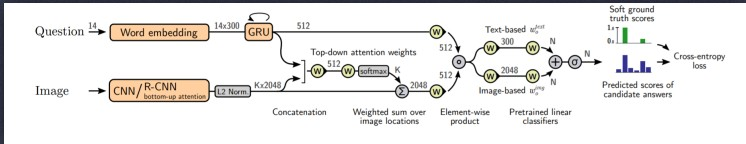
\includegraphics [width = 12cm, height= 3cm]{image/bab2/teney_model.jpeg}}
%     \caption{Teney Model \citep{srivastava2021visual}}
%     \label{exp: teney model}
% \end{figure}

\par VQA telah menarik minat besar dan mengalami perkembangan oleh para peneliti dan ilmuwan dari seluruh dunia. Tren terbaru yang diamati adalah dalam pengembangan \textit{dataset} yang terlihat semakin mirip dengan dunia nyata dengan menggabungkan pertanyaan dan jawaban seputar kehidupan nyata. Tren terkini juga terlihat dalam pengembangan model \textit{deep learning} yang lebih canggih dengan lebih baik memanfaatkan petunjuk visual dan petunjuk teks melalui berbagai cara. Kinerja model terbaik saat ini masih tertinggal dan hanya sekitar 60-70\% saja. Oleh karena itu, masih merupakan masalah yang terbuka untuk mengembangkan model \textit{deep learning} yang baik serta \textit{dataset} yang lebih menantang untuk \textit{visual question answering} \citep{srivastava2021visual}. 

\par Dalam mengembangkan sistem VQA diperlukan dua cabang ilmu seperti yang sudah dijelaskan yaitu \textit{computer vision} dan \textit{natural language processing} dikarenakan melibatkan gambar dan pertanyaan teks yang terkait \citep{teney2017visual}.

\subsection{\textit{Computer Vision}}

\par \textit{Computer Vision} (CV) bisa diartikan sebagai sekelompok teknik yang digunakan untuk mengumpulkan, memproses, menganalisis, dan memahami data yang kompleks dan berdimensi tinggi dari lingkungan sekitar kita. Tujuannya adalah untuk menjalani eksplorasi ilmiah dan teknis yang melibatkan pemahaman dan interpretasi data visual. Secara sederhana, CV memungkinkan komputer atau sistem komputasi untuk melihat, menginterpretasi, dan merespons informasi visual dari dunia nyata. Teknologi ini memiliki berbagai aplikasi, termasuk pengenalan objek, deteksi pola, dan pengolahan citra, serta mendukung berbagai bidang seperti kecerdasan buatan, penglihatan mesin, dan analisis data visual \citep{jahne1999handbook}.


\subsection{\textit{Natural Language Processing}}

\par \textit{Natural Language Processing} (NLP) adalah cabang ilmu dari pembelajaran mesin yang berfokus pada teks. Metode ini memungkinkan suatu komputer untuk menganalisis, memahami, dan menghasilkan makna dari bahasa manusia dengan cerdas dan bermanfaat. Dengan memanfaatkan NLP, pengembang dapat mengorganisir dan menyusun pengetahuan untuk menjalankan tugas-tugas seperti rangkuman otomatis, terjemahan, pengenalan entitas bernama, ekstraksi hubungan, analisis sentimen, pengenalan ucapan, dan segmentasi topik \citep{agarwal2019overview}.

\par Dalam NLP \textit{word embedding} merupakan representasi dari suatu kata. \textit{Embedding} digunakan dalam analisis teks. Biasanya, representasi tersebut berupa vektor nilai rill yang mengkodekan makna kata sedemikian rupa sehingga kata-kata yang lebih dekat dalam ruang vektor diharapkan memiliki makna yang mirip \citep{teller2000speech}. \textit{Global Vectors for Word Representation} (GloVe) adalah metode untuk membuat representasi kata. GloVe adalah algoritma \textit{unsupervised learning} yang memperoleh representasi vektor untuk kata-kata dengan melatih pada statistik kumulatif keterjadian bersama global kata-kata dari suatu korpus. Representasi yang dihasilkan menunjukkan struktur sublinear menarik dari ruang vektor kata, memungkinkan kata-kata dengan makna serupa berada lebih dekat dalam ruang vektor. Dalam hal ini, GloVe digunakan untuk membangun fitur \textit{embedding} kata semantik dan telah digunakan dalam berbagai tugas dalam bidang NLP \citep{pennington2014glove}.

\section{\textit{Medical Visual Question Answering Dataset}}

\par \textit{Medical visual question answering dataset} adalah \textit{dataset} yang digunakan untuk melakukan penelitian terkait tugas yang berkaitan dengan \textit{medical visual question answering} \citep{lin2023medical}. \textit{Dataset} ini berisi gambar medis dan pertanyaan yang terkait dengan gambar tersebut. Pada penelitian ini akan digunakan \textit{dataset} PathVQA dan VQA-RAD. Berikut adalah penjelasan dari kedua \textit{dataset} tersebut.

\subsection{PathVQA \textit{Dataset}}

\par \textit{Dataset} PathVQA berisi 32.799 pertanyaan dan jawaban dari 1.670 gambar patologi yang dikumpulkan dari dua buku patologi, yaitu '\textit{Textbook of Pathology}' dan '\textit{Basic Pathology}'. Selain itu, terdapat 3.328 gambar lainnya yang dikumpulkan dari perpustakaan digital PEIR. Dengan demikian, total gambar pada \textit{dataset} ini mencapai 4.998. Rata-rata setiap satu gambar memiliki 6,6 pertanyaan. Jumlah pertanyaan maksimal dan minimal adalah 14 dan 1 berturut-turut. Rata-rata jumlah kata per pertanyaan dan perjawaban adalah 9,5 dan 2,5 berturut-turut. Pada \textit{dataset} ini terdapat 7 kategori pertanyaan, yaitu: \textit{what}, \textit{where}, \textit{when}, \textit{whose}, \textit{how}, \textit{how much/how many}, dan \textit{yes/no}. Pertanyaan dari enam kategori pertama bersifat \textit{open-ended}, sedangkan pertanyaan dari kategori terakhir bersifat \textit{close-ended} '\textit{yes/no}'. Jumlah jawaban '\textit{yes}' dan '\textit{no}' adalah 8.145 dan 8.189 berturut-turut. Pertanyaan pada \textit{dataset} ini mencakup banyak aspek konten visual, termasuk warna, lokasi, penampilan, bentuk, dan lain-lain. Keragaman klinis ini menimbulkan tantangan yang besar bagi model AI dalam menjawab permasalahan pada gambar patologi \citep{xuehai2020pathvqa}.


\subsection{VQA-RAD \textit{Dataset}}

\par \textit{Dataset} VQA-RAD adalah \textit{dataset} yang dibuat secara manual untuk penelitian terkait \textit{Medical Visual Question Answering} (VQA). \textit{Dataset} ini berisi 3.515 pasangan pertanyaan dan jawaban yang dihasilkan oleh para klinisi, serta 315 gambar radiologi yang terbagi merata antara kepala, dada, dan perut. Dengan rata-rata, setiap gambar memiliki 10 pertanyaan terkait. Setiap gambar ini terkait dengan beberapa pertanyaan, yang dikelompokkan ke dalam 11 kategori: kelainan, atribut, modalitas, sistem organ, warna, penghitungan, keberadaan objek/kondisi, ukuran, bidang, penalaran posisional, dan lain-lain. Setengah dari pertanyaan pada \textit{dataset} ini bersifat \textit{close-ended} (\textit{yes/no}), sedangkan setengahnya lagi bersifat \textit{open-ended}. \textit{Dataset} ini merupakan kontribusi berharga dalam pengembangan model VQA di bidang radiologi, dengan pertanyaan-pertanyaan yang disusun oleh para ahli klinis, mencakup berbagai aspek interpretasi gambar medis \citep{lau2018dataset}.



\section{Penelitian Terkait}

\par Penelitian yang dilakukan oleh \citep{xuehai2020pathvqa} berhasil mengatasi tantangan khusus dalam analisis citra patologi dengan menggabungkan metode pemrosesan gambar dan pemrosesan bahasa alami. Mereka melakukan eksperimen dengan tiga metode berbeda. Tiga metode yang digunakan melibatkan integrasi \textit{Gated Recurrent Unit} (GRU) dan Faster R-CNN dengan melibatkan \textit{Bilinear Attention Network}, \textit{Convolutional Neural Network} (CNN) dan \textit{Long Short Term Memory} (LSTM) dengan \textit{compact bilinear pooling}, serta \textit{Stacked Attention Network} (SAN) yang menggabungkan CNN dan LSTM. Pengkodean gambar menggunakan Faster R-CNN dan ResNet-152. Berdasarkan ketiga eksperimen ini menunjukkan bahwa metode pertama mencapai akurasi tertinggi untuk pertanyaan \textit{close-ended} adalah 68,2\% dan mendapatkan nilai BLEU-1, BLEU-2, BLEU-3 sebesar 32,4, 22,8, 17,4 berturut-turut untuk pertanyaan \textit{open-ended}. Metode kedua mencapai akurasi sebesar 57,6\% untuk pertanyaan \textit{close-ended} dan mendapatkan BLEU-1, BLEU-2, BLEU-3, sebesar 13,3, 9,5, 6,8 berturut-turut untuk pertanyaan \textit{open-ended}. Metode ketiga mendapatkan akurasi sebesar 59,4\% untuk pertanyaan \textit{close-ended} dan mendapatkan BLEU-1, BLEU-2, BLEU-3 sebesar 19,2, 17,9, 15,8 berturut-turut untuk pertanyaan \textit{open-ended}. Lalu, hasil yang didapat ketika melakukan pengkodean gambar dengan Faster R-CNN mendapatkan akurasi 62,0\% untuk pertanyaan \textit{close-ended} dan mendapatkan BLEU-1, BLEU-2, BLEU-3 sebesar 24,7, 19,1, 16,5 berturut-turut untuk pertanyaan \textit{open-ended}. Sedangkan ketika menggunakan ResNet-152, mereka mendapatkan akurasi 60,1\% untuk pertanyaan \textit{close-ended} dan BLEU-1, BLEU-2, BLEU-3 sebesar 19,9, 18,0, 16,0 berturut-turut untuk pertanyaan \textit{open-ended} \citep{xuehai2020pathvqa}.

\par Penelitian lain juga dilakukan untuk meningkatkan diagnosis dengan menjawab pertanyaan klinis yang disajikan dengan gambar medis menggunakan model \textit{Contrastive Language Image Pre Training} (CLIP) yang mengintegrasikan pembelajaran \textit{multimodal embedding} melalui pelatihan bersama \textit{image encoder} dan \textit{text encoder} untuk memaksimalkan kemiripan pasangan gambar-teks yang sesuai. Metodenya melibatkan penggunaan \textit{Vision Transformer} (ViT) untuk \textit{image encoder}, pertanyaan dimasukkan ke dalam transformer \textit{encoder} teks, dan penggabungan representasi visual dan teks dalam \textit{decoder multimodal} untuk menghasilkan jawaban otomatis. Uji coba dilakukan pada dua \textit{dataset} VQA, PathVQA dan VQA-RAD, dengan konfigurasi menggunakan \textit{multi-head attention} sebesar 512, tingkat \textit{dropout} pada \textit{fully connected layers} 0,1, dan dua blok transformer pada \textit{encoder} dan \textit{decoder}. Fungsi optimasi yang digunakan adalah Adam dengan \textit{learning rate} 0,001, \textit{batch size} 50, dan 50 \textit{epoch} pelatihan, dengan citra diacak dan pengolahan teks menggunakan \textit{bert-base-uncased}. Hasilnya menunjukkan akurasi yang signifikan, dengan akurasi tertinggi mencapai 84,63\% untuk pertanyaan \textit{close-ended} dan akurasi, BLEU-1, BLEU-2, BLEU-3 adalah sebesar 58,29\% 61,78, 61,16, 59,28 secara berturut-turut untuk pertanyaan \textit{open-ended} dalam \textit{dataset} PathVQA. Pada \textit{dataset} VQA-RAD akurasi yang didapatkan adalah 82,47\% untuk pertanyaan \textit{close-ended} dan akurasi, BLEU-1, BLEU-2, BLEU-3 adalah sebesar 71,49\% 71,03, 70,81, 67,01 untuk pertanyaan \textit{open-ended} \citep{bazi2023vision}.




% \par Penelitian yang dilakukan oleh \citep{aioz_mevf_miccai19}, mereka mengemukakan sebuah konsep baru dalam bidang VQA medis yang memanfaatkan teknologi MAML (\textit{model-agnostic meta learning}) dan CDAE (\textit{convolutional denoising autoencoder}) untuk mengekstraksi fitur gambar. Hal ini bertujuan untuk mengatasi keterbatasan data pelatihan yang berlabel. Secara lebih rinci, CDAE membantu dalam mengambil manfaat dari informasi yang terdapat di dalam gambar yang tidak memiliki label dalam jumlah besar, Sementara MAML membantu dalam mempelajari bobot meta yang dapat dengan cepat diadaptasi untuk permasaflahan \textit{visual question answering}. Hasil eksperimen ini menunjukkan pencapaian baru yang sangat baik pada \textit{dataset} VQA-RAD, baik dalam hal pertanyaan yang bersifat \textit{open-ended} maupun \textit{close-ended}.

% \par Penelitian yang dilakukan oleh \citep{aioz_mmq_miccai21}, mereka mengusulkan metode baru untuk mengukur beberapa meta-model secara efektif dalam rangka memanfaatkan meta-anotasi dan mengatasi label yang tidak akurat dalam tugas VQA medis. Hasil eksperimen yang melibatkan sejumlah besar data menunjukkan bahwa metode yang dihasilkan dari penelitian ini jauh lebih unggul dibandingkan dengan metode berbasis meta-learning terkini dalam kedua \textit{dataset} PathVQA dan VQA-RAD. 



% \fancyhf{}
% \fancyfoot[R]{\thepage}

\begin{comment}
\bibliography{daftar-pustaka}
\end{comment}
